% Created 2022-03-15 Tue 15:46
% Intended LaTeX compiler: pdflatex
\documentclass[11pt]{article}
\usepackage[utf8]{inputenc}
\usepackage[T1]{fontenc}
\usepackage{graphicx}
\usepackage{grffile}
\usepackage{longtable}
\usepackage{wrapfig}
\usepackage{rotating}
\usepackage[normalem]{ulem}
\usepackage{amsmath}
\usepackage{textcomp}
\usepackage{amssymb}
\usepackage{capt-of}
\usepackage{hyperref}
\usepackage{minted}
\usepackage[margin=0.8in]{geometry}
\author{Mahan Fathi}
\date{\today}
\title{\textbf{Homework \#3}}
\hypersetup{
 pdfauthor={Mahan Fathi},
 pdftitle={\textbf{Homework \#3}},
 pdfkeywords={},
 pdfsubject={},
 pdfcreator={Emacs 27.2 (Org mode 9.5)}, 
 pdflang={English}}
\begin{document}

\maketitle
\clearpage
\section{Question 1}
\label{sec:orga1d818e}
\begin{figure}[htbp]
\centering
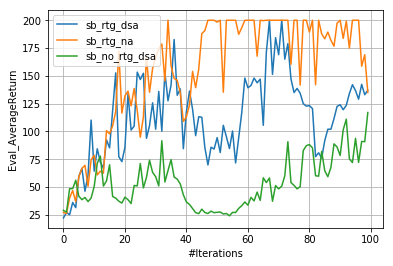
\includegraphics[width=.9\linewidth]{./q11.png}
\caption{\textbf{Q1} \texttt{CartPole-v0} with short \texttt{batch\_size=1000}}
\end{figure}

\begin{figure}[htbp]
\centering
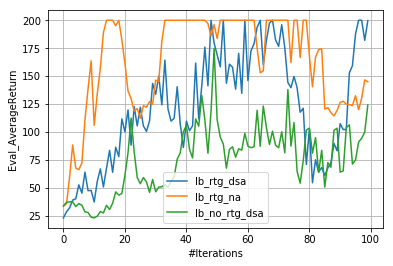
\includegraphics[width=.9\linewidth]{./q12.png}
\caption{\textbf{Q1} \texttt{CartPole-v0} with large \texttt{batch\_size=5000}}
\end{figure}

\begin{listing}[htbp]
\begin{minted}[]{bash}
python run_hw3.py env_name=CartPole-v0 n_iter=100 batch_size=1000 rl_alg=reinforce \
    estimate_advantage_args.standardize_advantages=false \
    exp_name=q1_sb_no_rtg_dsa estimate_advantage_args.reward_to_go=false
python run_hw3.py env_name=CartPole-v0 n_iter=100 batch_size=1000 rl_alg=reinforce \
    estimate_advantage_args.standardize_advantages=false \
    exp_name=q1_sb_rtg_dsa estimate_advantage_args.reward_to_go=true
python run_hw3.py env_name=CartPole-v0 n_iter=100 batch_size=1000 rl_alg=reinforce \
    estimate_advantage_args.standardize_advantages=true \
    exp_name=q1_sb_rtg_na estimate_advantage_args.reward_to_go=true
python run_hw3.py env_name=CartPole-v0 n_iter=100 batch_size=5000 rl_alg=reinforce \
    estimate_advantage_args.standardize_advantages=false \
    exp_name=q1_lb_no_rtg_dsa estimate_advantage_args.reward_to_go=false
python run_hw3.py env_name=CartPole-v0 n_iter=100 batch_size=5000 rl_alg=reinforce \
    estimate_advantage_args.standardize_advantages=false \
    exp_name=q1_lb_rtg_dsa estimate_advantage_args.reward_to_go=true
python run_hw3.py env_name=CartPole-v0 n_iter=100 batch_size=5000 rl_alg=reinforce \
    estimate_advantage_args.standardize_advantages=true \
    exp_name=q1_lb_rtg_na estimate_advantage_args.reward_to_go=true
\end{minted}
\caption{\textbf{Q1} Run commands}
\end{listing}

\begin{itemize}
\item Questions:
\begin{itemize}
\item \texttt{rtg} is outperforming naive REINFORCE as expected. Using reward-to-go reduces the variance of the gradient estimator, at no cost (unbiased).
\item Standardizing helps regardless of the batch size.
\item Using a larger batch size helps a lot with the convergence rate -- 5x \texttt{batch\_size} roughly speeds up convergence by 2x.
\end{itemize}
\end{itemize}


\clearpage

\section{Question 2}
\label{sec:orgff4af76}

\begin{figure}[htbp]
\centering
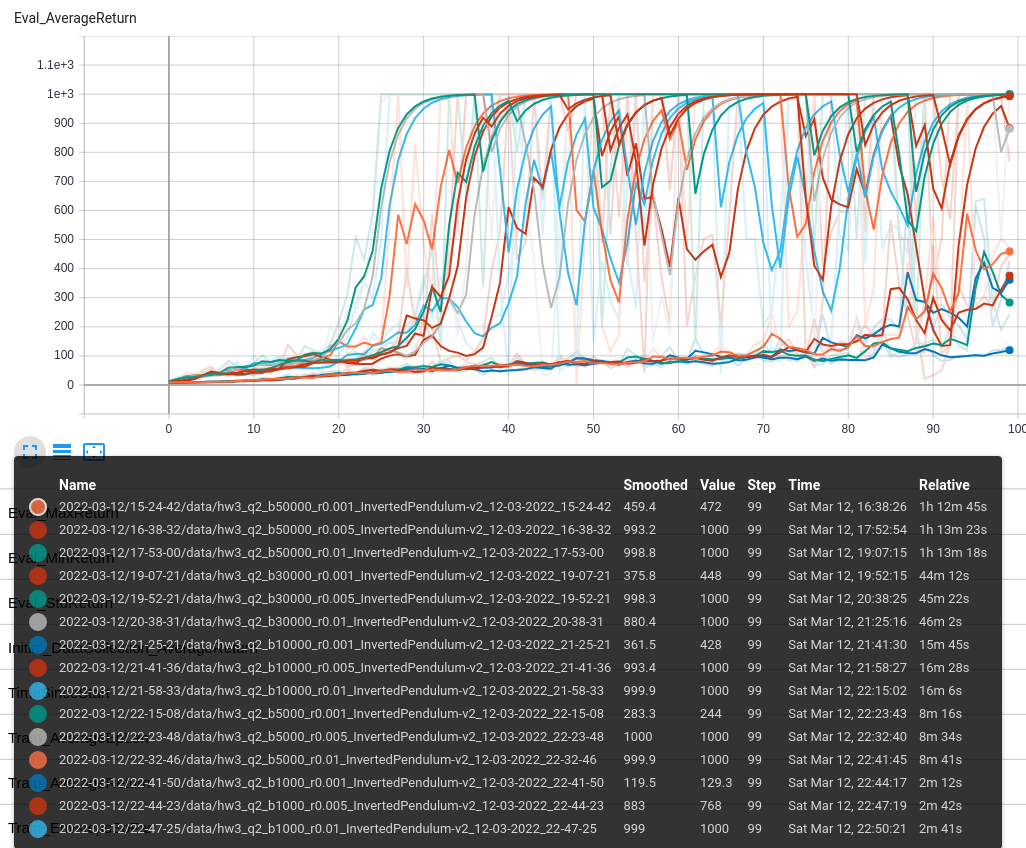
\includegraphics[width=.9\linewidth]{./q2.png}
\caption{\textbf{Q2} \texttt{InvertedPendulum-v2} search}
\end{figure}

\begin{table}[htbp]
\caption{\textbf{Q2} results}
\centering
\begin{tabular}{l|r|r}
\hline
* & \texttt{batch\_size} & \texttt{learning\_rate}\\
\hline
Fastest convergence & 50000 & 0.01\\
\hline
min \texttt{batch\_size} & 1000 & -\\
\hline
min \texttt{learning\_rate} & - & 0.01\\
\hline
min \texttt{lr} and \texttt{bs} & 1000 & 0.01\\
\hline
\end{tabular}
\end{table}

Since \texttt{InvertedPendulum-v2} uses a continuous reward function (penalizes for deviations from the center, i.e. a properly shaped reward), we can use much lower batch sizes.

\begin{listing}[htbp]
\begin{minted}[]{bash}
for batch_size in 50000 30000 10000 5000 1000; do
    for learning_rate in 0.001 0.005 0.01; do
        echo "BATCH_SIZE=$batch_size, LR=$learning_rate"
        python run_hw3.py env_name=InvertedPendulum-v2 \
            n_iter=100 ep_len=1000 computation_graph_args.n_layers=3 \
            computation_graph_args.size=64 \
            train_batch_size=$batch_size batch_size=$batch_size \
            batch_size_initial=$batch_size \
            computation_graph_args.learning_rate=$learning_rate \
            estimate_advantage_args.standardize_advantages=true \
            exp_name=q2_b${batch_size}_r${learning_rate} \
            estimate_advantage_args.reward_to_go=true rl_alg=reinforce
    done
done
\end{minted}
\caption{\textbf{Q2} Run commands}
\end{listing}

\clearpage
\section{Question 3}
\label{sec:org302d208}
My lunar lander does not converge sadly, and I tried so many things and trust my implementation, but I have just given up. In the best cases it would get close to zero, and then just collapses afterwards.

\begin{figure}[htbp]
\centering
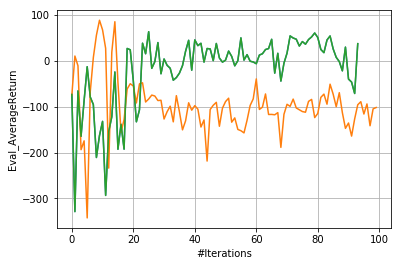
\includegraphics[width=.9\linewidth]{./3.png}
\caption{\textbf{Q3} Failed attempts at \texttt{LunarLanderContinuous-v2}}
\end{figure}

\begin{listing}[htbp]
\begin{minted}[]{bash}
python run_hw3.py env_name=LunarLanderContinuous-v2 no_gpu=True n_iter=100 \
    ep_len=1000 computation_graph_args.n_layers=2 computation_graph_args.size=64 \
    estimate_advantage_args.discount=0.99 batch_size=40000 train_batch_size=40000 \
    batch_size_initial=40000 computation_graph_args.learning_rate=0.005 \
    estimate_advantage_args.nn_baseline=true \
    estimate_advantage_args.standardize_advantages=false \
    exp_name="q3_b100000_r0.003" estimate_advantage_args.reward_to_go=true \
    rl_alg=reinforce estimate_advantage_args.gae_lambda=false seed=7
# as a desperate measure I also tried changing the seed :(
\end{minted}
\caption{\textbf{Q3} Run commands}
\end{listing}

\clearpage
\section{Question 4}
\label{sec:orgd120cc7}


\begin{figure}[htbp]
\centering
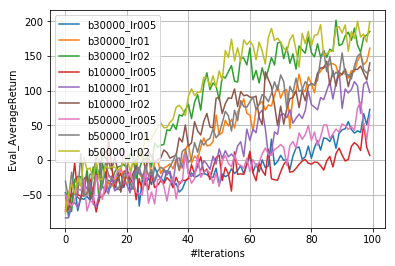
\includegraphics[width=.9\linewidth]{./41.png}
\caption{\textbf{Q4} Hyperparam search for \texttt{HalfCheetah-v2}}
\end{figure}

Increasing the batch size does not necessarily helps with the convergence rate, but it checks out with the overall pattern. Using a larger bach size leads to lower variance in general. As to how the learning rate affects the convergence, it basically boils down to the magnitude of the step to take in the direction suggested based on the data, which is of size \texttt{batch\_size}. So given the right direction, i.e. assuming we have minimal variance in the gradient estimator, we can treat the problem as a supervised learning problem, and \(0.02\) seems like the perfect step size for that.

\begin{figure}[htbp]
\centering
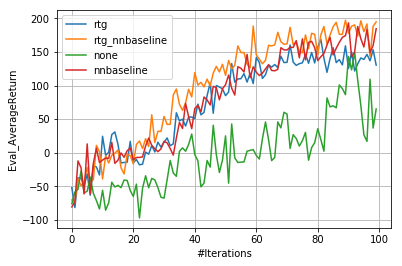
\includegraphics[width=.9\linewidth]{./42.png}
\caption{\textbf{Q4} \texttt{HalfCheetah-v2} with/without \texttt{rtg/nnbaseline}}
\end{figure}

\begin{listing}[htbp]
\begin{minted}[]{bash}
for batch_size in 30000 10000 50000; do
    for learning_rate in 0.005 0.01 0.02; do
        echo "BATCH_SIZE=$batch_size, LR=$learning_rate"
        python run_hw3.py env_name=HalfCheetah-v2 n_iter=100 ep_len=150 \
            computation_graph_args.n_layers=2 computation_graph_args.size=32 \
            estimate_advantage_args.discount=0.95 train_batch_size=$batch_size \
            batch_size=$batch_size batch_size_initial=$batch_size \
            computation_graph_args.learning_rate=$learning_rate \
            estimate_advantage_args.nn_baseline=true \
            estimate_advantage_args.standardize_advantages=true \
            exp_name="q4_search_b${batch_size}_lr${learning_rate}_rtg_nnbaseline" \
            estimate_advantage_args.reward_to_go=true rl_alg=reinforce
    done
done

batch_size=50000
learning_rate=0.02
python run_hw3.py env_name=HalfCheetah-v2 n_iter=100 ep_len=150 \
    computation_graph_args.n_layers=2 computation_graph_args.size=32 \
    estimate_advantage_args.discount=0.95 train_batch_size=$batch_size \
    batch_size=$batch_size batch_size_initial=$batch_size \
    computation_graph_args.learning_rate=$learning_rate \
    estimate_advantage_args.nn_baseline=false \
    estimate_advantage_args.standardize_advantages=true \
    exp_name="q4_b${batch_size}_lr${learning_rate}" \
    estimate_advantage_args.reward_to_go=false rl_alg=reinforce

python run_hw3.py env_name=HalfCheetah-v2 n_iter=100 ep_len=150 \
    computation_graph_args.n_layers=2 computation_graph_args.size=32 \
    estimate_advantage_args.discount=0.95 train_batch_size=$batch_size \
    batch_size=$batch_size batch_size_initial=$batch_size \
    computation_graph_args.learning_rate=$learning_rate \
    estimate_advantage_args.nn_baseline=false \
    estimate_advantage_args.standardize_advantages=true \
    exp_name="q4_b${batch_size}_lr${learning_rate}_rtg" \
    estimate_advantage_args.reward_to_go=true rl_alg=reinforce

\end{minted}
\caption{\textbf{Q4} Run commands (1/2)}
\end{listing}

\begin{listing}[htbp]
\begin{minted}[]{bash}
python run_hw3.py env_name=HalfCheetah-v2 n_iter=100 ep_len=150 \
    computation_graph_args.n_layers=2 computation_graph_args.size=32 \
    estimate_advantage_args.discount=0.95 train_batch_size=$batch_size \
    batch_size=$batch_size batch_size_initial=$batch_size \
    computation_graph_args.learning_rate=$learning_rate \
    estimate_advantage_args.nn_baseline=true \
    estimate_advantage_args.standardize_advantages=true \
    exp_name="q4_b${batch_size}_lr${learning_rate}_nnbaseline" \
    estimate_advantage_args.reward_to_go=false rl_alg=reinforce

python run_hw3.py env_name=HalfCheetah-v2 n_iter=100 ep_len=150 \
    computation_graph_args.n_layers=2 computation_graph_args.size=32 \
    estimate_advantage_args.discount=0.95 train_batch_size=$batch_size \
    batch_size=$batch_size batch_size_initial=$batch_size \
    computation_graph_args.learning_rate=$learning_rate \
    estimate_advantage_args.nn_baseline=true \
    estimate_advantage_args.standardize_advantages=true \
    exp_name="q4_b${batch_size}_lr${learning_rate}_rtg_nnbaseline" \
    estimate_advantage_args.reward_to_go=true rl_alg=reinforce
\end{minted}
\caption{\textbf{Q4} Run commands (2/2)}
\end{listing}

\clearpage
\section{Question 5}
\label{sec:org65f1a97}

\begin{figure}[htbp]
\centering
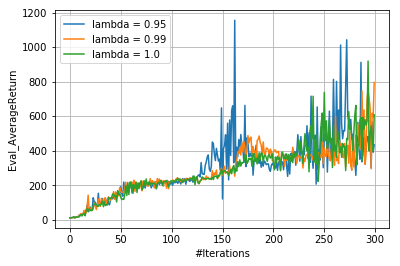
\includegraphics[width=.9\linewidth]{./5.png}
\caption{\textbf{Q5} GAE-\(\lambda\) search for \texttt{Hopper-v2}}
\end{figure}

\begin{listing}[htbp]
\begin{minted}[]{bash}
batch_size=2000
learning_rate=0.001
for lambda in 0.95 0.99 1.0; do
    python run_hw3.py env_name=Hopper-v2 n_iter=300 ep_len=1000 \
        computation_graph_args.n_layers=2 computation_graph_args.size=32 \
        estimate_advantage_args.discount=0.99 train_batch_size=$batch_size \
        batch_size=$batch_size batch_size_initial=$batch_size \
        computation_graph_args.learning_rate=$learning_rate \
        estimate_advantage_args.nn_baseline=true \
        estimate_advantage_args.standardize_advantages=true \
        estimate_advantage_args.gae_lambda=$lambda \
        exp_name="q5_b${batch_size}_r${learning_rate}_lambda${lambda}" \
        estimate_advantage_args.reward_to_go=true rl_alg=reinforce
done
\end{minted}
\caption{\textbf{Q5} Run commands}
\end{listing}

\clearpage
\section{Question 6}
\label{sec:org5d56b78}

\begin{figure}[htbp]
\centering
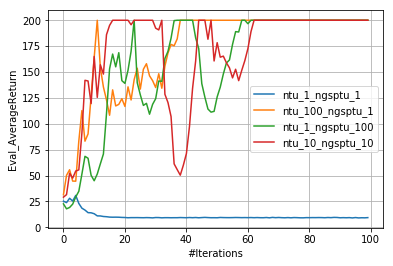
\includegraphics[width=.9\linewidth]{./6.png}
\caption{\textbf{Q6} \texttt{\#ntu/\#ngsptu} search for \texttt{CartPole-v0}}
\end{figure}

Verdict: \texttt{ntu, ngsptu = 10, 10} works best.

\begin{listing}[htbp]
\begin{minted}[]{bash}
batch_size=1000
for ntu in 1 10 100; do
    for ngsptu in 1 10 100; do
        python run_hw3.py env_name=CartPole-v0 n_iter=100 \
            rl_alg=ac train_batch_size=$batch_size \
            batch_size=$batch_size batch_size_initial=$batch_size \
            estimate_advantage_args.nn_baseline=true \
            estimate_advantage_args.standardize_advantages=true \
            estimate_advantage_args.reward_to_go=true \
            exp_name="q6_ac_${ntu}_${ngsptu}" \
            computation_graph_args.num_target_updates=$ntu \
            computation_graph_args.num_grad_steps_per_target_update=$ngsptu
    done
done
\end{minted}
\caption{\textbf{Q6} Run commands}
\end{listing}


\clearpage
\section{Question 7}
\label{sec:org666db8e}

\begin{figure}[htbp]
\centering
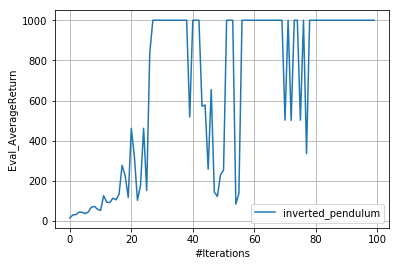
\includegraphics[width=.9\linewidth]{./71.png}
\caption{\textbf{Q7} AC for \texttt{InvertedPendulum-v2}}
\end{figure}

\begin{listing}[htbp]
\begin{minted}[]{bash}
batch_size=5000
python run_hw3.py env_name=InvertedPendulum-v2 n_iter=100 ep_len=1000 \
    computation_graph_args.n_layers=2 computation_graph_args.size=64 \
    train_batch_size=$batch_size batch_size=$batch_size \
    batch_size_initial=$batch_size \
    computation_graph_args.learning_rate=0.01 \
    estimate_advantage_args.nn_baseline=true \
    estimate_advantage_args.standardize_advantages=true \
    exp_name="q7_10_10" estimate_advantage_args.reward_to_go=true \
    rl_alg=ac computation_graph_args.num_target_updates=10 \
    computation_graph_args.num_grad_steps_per_target_update=10
\end{minted}
\caption{\textbf{Q7} Run commands (1/2)}
\end{listing}

\begin{figure}[htbp]
\centering
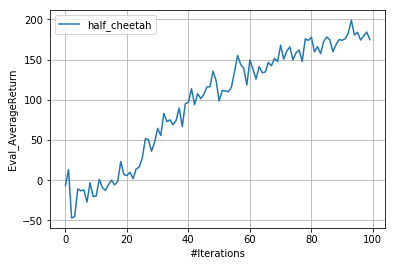
\includegraphics[width=.9\linewidth]{./72.png}
\caption{\textbf{Q7} AC for \texttt{HalfCheetah-v2}}
\end{figure}

\begin{listing}[htbp]
\begin{minted}[]{bash}
batch_size=30000
python run_hw3.py env_name=HalfCheetah-v2 n_iter=100 ep_len=150 \
    computation_graph_args.n_layers=2 computation_graph_args.size=32 \
    train_batch_size=$batch_size batch_size=$batch_size \
    batch_size_initial=$batch_size computation_graph_args.learning_rate=0.02 \
    eval_batch_size=1500 estimate_advantage_args.discount=0.9 \
    estimate_advantage_args.nn_baseline=true \
    estimate_advantage_args.standardize_advantages=true \
    exp_name="q7_10_10" estimate_advantage_args.reward_to_go=true \
    rl_alg=ac computation_graph_args.num_target_updates=10 \
    computation_graph_args.num_grad_steps_per_target_update=10
\end{minted}
\caption{\textbf{Q7} Run commands (2/2)}
\end{listing}

\clearpage
\section{Question 8}
\label{sec:orgb553675}
Description of the implementation: I am using dyna models to imagine full-blown trajectories; first I train the models using \uline{randomly} sampled data from the replay buffer, then I sample \uline{recent} data, which gives me full trajectories that I can use to form policy gradient updates, however, I also concatenate these trajectories with the imagined ones via dyna models, which are also reward labled using \texttt{self.env.get\_reward()}. The results are not great, but this was my understanding of dyna.

\begin{figure}[htbp]
\centering
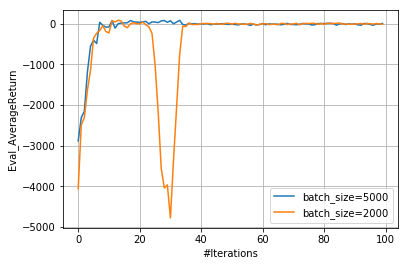
\includegraphics[width=.9\linewidth]{./8.png}
\caption{\textbf{Q8} Dyna for \texttt{HalfCheetah-v2}}
\end{figure}

\begin{listing}[htbp]
\begin{minted}[]{bash}
batch_size=5000
python run_hw3.py env_name=cheetah-ift6163-v0 n_iter=100 \
    computation_graph_args.n_layers=2 computation_graph_args.size=32 \
    estimate_advantage_args.discount=0.95 train_batch_size=$batch_size \
    batch_size=$batch_size batch_size_initial=$batch_size \
    computation_graph_args.learning_rate=0.01 \
    estimate_advantage_args.nn_baseline=true \
    estimate_advantage_args.standardize_advantages=true \
    exp_name="q8_cheetah_n500-arch1x32" \
    estimate_advantage_args.reward_to_go=true rl_alg=dyna

batch_size=2000
python run_hw3.py env_name=cheetah-ift6163-v0 n_iter=100 \
    computation_graph_args.n_layers=2 computation_graph_args.size=32 \
    estimate_advantage_args.discount=0.95 train_batch_size=$batch_size \
    batch_size=$batch_size batch_size_initial=$batch_size \
    computation_graph_args.learning_rate=0.01 \
    estimate_advantage_args.nn_baseline=true \
    estimate_advantage_args.standardize_advantages=true \
    exp_name="q8_cheetah_n500-arch1x32" \
    estimate_advantage_args.reward_to_go=true rl_alg=dyna
\end{minted}
\caption{\textbf{Q8} Run commands}
\end{listing}
\end{document}
